\documentclass{standalone}
\usepackage{hsbcommon}
\begin{document}
       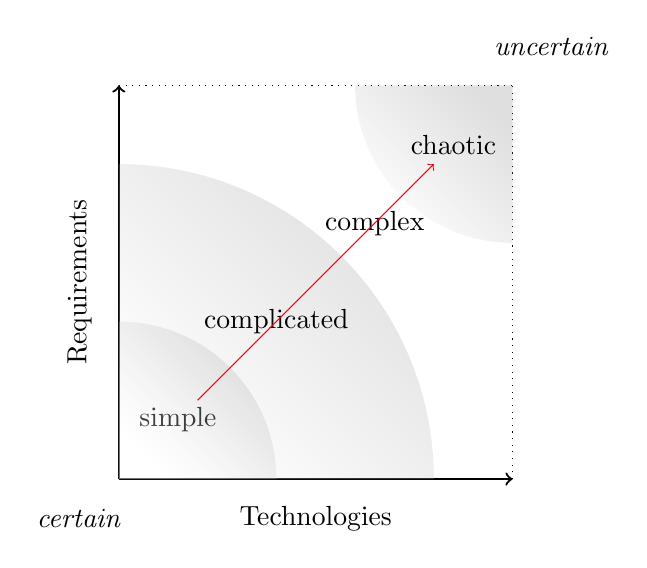
\begin{tikzpicture}[scale=1]  %% requires tikz
          \draw[thick,->] (0,0) -- (5,0);
          \node (x) at (5.5,5.5) {\emph{uncertain}};
          \node[rotate=90] (r) at (-.5,2.5) {Requirements};
          \draw[thick,->] (0,0) -- (0,5); 
          %\node (y) at (0,5.5) {$uncertainty$};
          \node (r) at (2.5,-0.5) {Technologies};
          \draw[dotted] (0,5) -- (5,5) ;
          \draw[dotted] (5,0) -- (5,5) ;
          \node (o) at (-.5,-.5) {\emph{certain}} ;
         \shade [shading angle=-45, opacity=.25] (2,0,0) arc (0:90:2) -- (0,0,0) -- cycle;
         \node (e) at (0.75,0.75) {simple};
          \shade [shading angle=-45, opacity=.25] (4,0,0) arc (0:90:4) -- (0,0,0) -- cycle;
          \node (e) at (2,2) {complicated};
          \node (e) at (3.25,3.25) {complex};
          \shade [shading angle=-45, opacity=.25] (3,5,0) arc (180:270:2) -- (5,5,0) -- cycle;
          \node (e) at (4.25,4.25) {chaotic};
          \draw[color=red, ->] (1,1) -- (4,4) ;
        \end{tikzpicture}   

\end{document}
